\chapter{Power Measurement}

\section{Validating RAPL Accuracy}
\todoms{Add references}
Starting with the Haswell microarchitecture Intel integrated current measurement into their processor to support power limiting.
The associated power metrics for differenet zones can be measured using the RAPL interface via the linux kernel.
Schöne et al. tried to validate RAPL accuracy for the Alder Lake architecture, which also uses the Golden Cove core microarchitecture.
They revealed that the power measurement is not accurate on this specific architecture.
This requires me to replicate the measurement and check if the RAPL measurement is accurate.

I run the roco2 synthetic workload generator on the test system.
The software required some patches.
They are documented in the forked GitHub repository~\footnote{\url{https://github.com/marenz2569/roco2/tree/marenz.hati-config}}.

Each of the displayed workload in~\figref{validate-rapl} were run for \SI{60}{\second} on the cross product of following settings:
\begin{itemize}
    \item Maximal core frequency set to \SI{800}{\MHz}, \SI{2000}{\MHz} and \SI{3800}{\MHz} (turbo).
    \item Lowest enabled C-states of \texttt{POLL}, \texttt{C1} and \texttt{C2}.
    \item Four different number of cores all on the same socket \SI{14}{}, \SI{28}{}, \SI{42}{} and \SI{56}{}.
\end{itemize}
The test matrix further included a full idle for each C-state setting.
Hyperthreading was disabled and the governor set to \texttt{performance}.
The power metrics were measured through the FIRESTARTER measurement inferface.
This polls the RAPL metrics every \SI{10}{\ms} and discovered the first and last \SI{5}{\second} of each measurement duration.
The reference measurent of the PDU is exposed via the metricq metric inferface and reports \SI{1}{Sa\per\second}.
The average of both metrics is plotted in~\figref{validate-rapl}.
This shows us a strong correlation via the quadratic fit.
All measurment points are inside the \SI{1}{\percent} tolerance of the PDU.

\begin{figure}[]
    \centering
    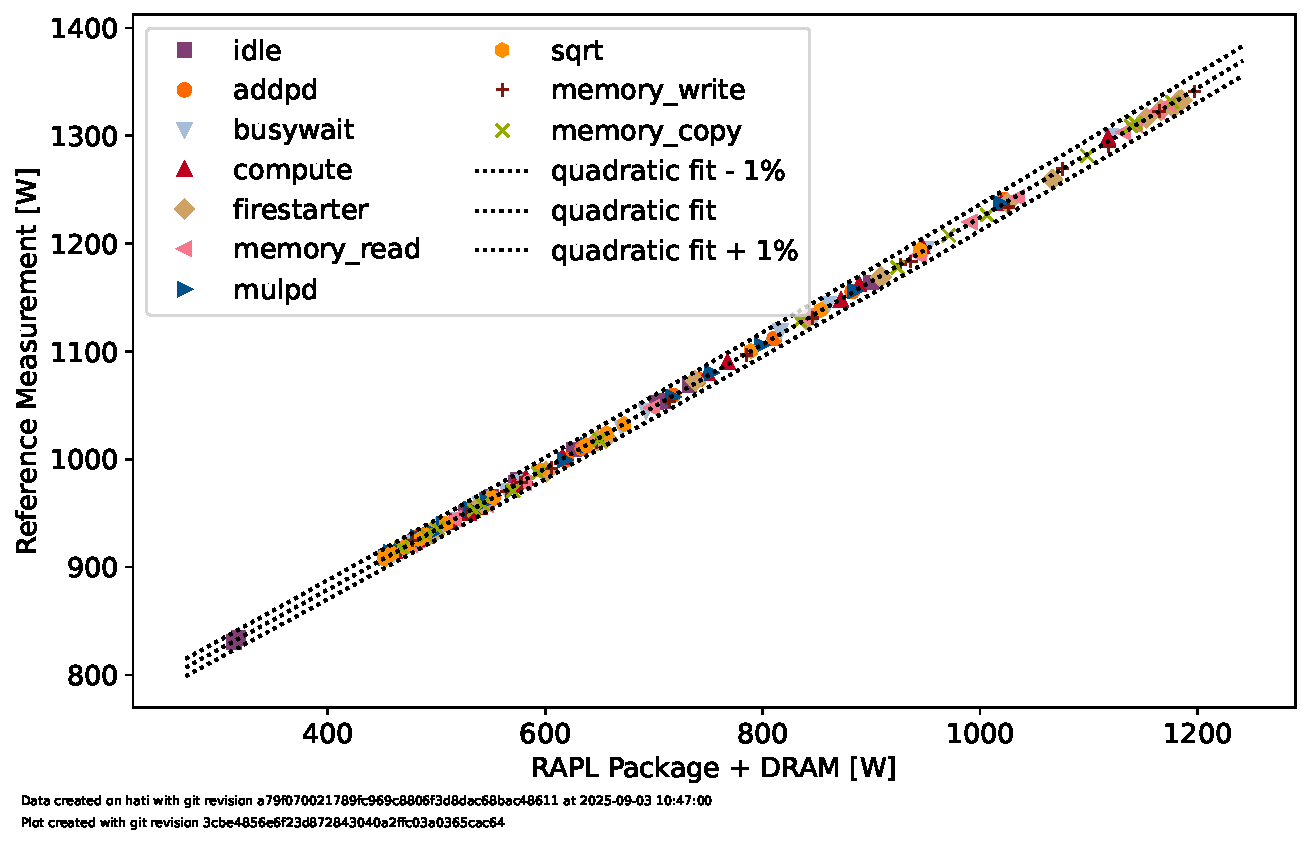
\includegraphics[width=0.8\columnwidth]{fig/rapl-accuracy/rapl-accuracy.pdf}
    \caption{\label{fig:validate-rapl}The roco2 microbenchmark is executed on a varying number of cores with different frequencies.
    The RAPL measurement can be mapped with a quadratic fit to the external measurement.}
\end{figure}

\section{RAPL Filters}

\todoms{Influence of the data on the RAPL measurements.}
\todoms{Influence of the measurement time on the RAPL measurements.}
